\chapter{Polytope representation of physical abilities} % Main chapter title
\label{ch:phisical_ability_metrics} 

As described in the introduction chapter, polytope based representations of different physical abilities (physical ability polytopes) of humans and robots enable an accurate characterisation of their individual abilities. Furthermore, by expressing their individual abilities in the polytope form, their common abilities when collaborating can be computed using efficient polytope algebra operations and represented in polytope form as well. 
Numerous polytope-based physical ability characterisations have been developed in the literature, both for humans and robots. Therefore, the aim of this chapter is to present an overview of the common physical ability polytopes, applicable to both humans and robots, in the attempt to propose an unified vision of their individual abilities.  

\Cref{ch:robot_metrics} brings an overview of the common polytope formulations for robotic manipulators, while \Cref{ch:human_metrics} presents the common metrics for humans, based on their musculoskeletal models. 
\Cref{ch:collab_metrics} then discusses using different polytope algebra operators to calculate the joint physical abilities of humans and robots when engaged in physical interactions to accomplish specific tasks.
Finally, the \Cref{ch:collab_metrics_overview} concludes the chapter and provides a structured synthesis of common polytope formulations, proposing a single generic polytope formulation encompassing all the common formulations for both humans and robots.

\section{Physical ability polytope formulations for robotic manipulators}
\label{ch:robot_metrics}

Physical ability characterisations based on polytopes are most accurate local, state dependent, metrics for the performance analysis of robotic systems \cite{pholsiri2005real,Finotello1998}. They describe a mapping between the robot's actuator limits (torques, accelerations , velocities, etc.) and the limits of different task space variables (wrenches, accelerations, velocities, etc.) . 

The aim of this section is to provide an overview of common polytope formulations for robotic systems in an unified view.  Therefore, \Cref{ch:robot_dyn_kin} bringing a quick overview of the dynamics and kinematics equations for robotic systems, used for different polytope definitions. Definitions 
of common polytope characterisations of physical abilities are then described in subsequent sections (\Cref{ch:vel_poly} - \ref{ch:human_stiffness_poly}).

\subsection{Dynamics and kinematics relationships}
\label{ch:robot_dyn_kin}
The actuation limits, of a robotic manipulator with $n$ joints, are commonly specified as independent ranges of achievable actuator positions $\bm{q}\in \mathbb{R}^n$, velocities $\dot{\bm{q}}\in \mathbb{R}^n$, actuator torques $\bm{\tau}\in \mathbb{R}^n$ and sometimes even torque derivatives $\dot{\bm{\tau}}\in \mathbb{R}^n$.
\begin{subequations}
\begin{align}
\bm{q} &\in [ {\bm{q}}_{min}, {\bm{q}}_{max}], \quad\dot{\bm{q}} \in [\dot{\bm{q}}_{min},  \dot{\bm{q}}_{max}], \\
\quad\bm{\tau} &\in [\bm{\tau}_{min},  \bm{\tau}_{max}],
\quad\dot{\bm{\tau}} \in [\dot{\bm{\tau}}_{min},  \dot{\bm{\tau}}_{max}] \label{eq:dyn_limits:torque}
\end{align}
\label{eq:dyn_limits}
\end{subequations}
The dynamical model, of a standard serial robotic manipulator with a fixed base, is commonly defined as
\begin{equation}
M(\bm{q})\ddot{\bm{q}} + C(\bm{q},\dot{\bm{q}})\dot{\bm{q}} + \bm{g}(\bm{q}) + J^T(\bm{q})\bm{f} = \bm{\tau} 
\label{eq:dyn_model_rob}
\end{equation}
where $M(\bm{q}) \in \mathbb{R}^{n \times n}$ and $C(\bm{q},\dot{\bm{q}})\in \mathbb{R}^{n \times n}$ are the inertia and Coriolis matrices, $\bm{g} (\bm{q})\in \mathbb{R}^n$ is the state dependent gravity vector, $J(\bm{q}) \in \mathbb{R}^{m\times n}$ is the state dependant Jacobian matrix, $\bm{f}\in \mathbb{R}^m $ is the vector of applied external wrenches and $\bm{q},\dot{\bm{q}},\ddot{\bm{q}}$ are robot's joint positions, velocities and accelerations respectively.

Furthermore, the mapping between the $n$ dimensional space of robot's actuator (joint) positions $\bm{q}\in \mathbb{R}^n$ and the $m$ dimensional task space positions $\bm{x} \in \mathbb{R}^m$ can be found through the robot's forward kinematics 
\begin{equation}
    \bm{x} = \fk{\bm{q}}
\end{equation}
whereas the task space velocity $\dot{\bm{x}}\in \mathbb{R}^m$, acceleration $\ddot{\bm{x}}\in \mathbb{R}^m$ and jerk $\dddot{\bm{x}}\in \mathbb{R}^m$ can be found through the state dependent  $\{\bm{q},\dot{\bm{q}},\ddot{\bm{q}}\}$  and nonlinear mapping
\begin{subequations}
\begin{align}
\dot{\bm{x}}&= {J}(\bm{q})\dot{\bm{q}} \label{eq:js_to_cs_vaj:vel}\\
\ddot{\bm{x}}&= J(\bm{q})\ddot{\bm{q}} + \dot{J}(\bm{q},\dot{\bm{q}})\dot{\bm{q}} \label{eq:js_to_cs_vaj:accel}\\
\dddot{\bm{x}}&= J(\bm{q})\dddot{\bm{q}} + 2\dot{J}(\bm{q},\dot{\bm{q}})\ddot{\bm{q}} + \ddot{J}(\bm{q},\dot{\bm{q}},\ddot{\bm{q}})\dot{\bm{q}}\label{eq:js_to_cs_vaj:jerk}
 \end{align} \label{eq:js_to_cs_vaj}
\end{subequations}
were $J(\bm{q}) $ is the Jacobian matrix
\begin{equation}
    J(\bm{q}) = \frac{\partial \fk{\bm{q}}}{\partial \bm{q}}
\end{equation}
while $\dot{J}(\bm{q},\dot{\bm{q}})$ and $\ddot{J}(\bm{q},\dot{\bm{q}},\ddot{\bm{q}})$ are its first and second time derivatives.


It is worth noting that in general case, $m$ dimensional task space might include positions and orientations, for example if the task space corresponds to the \gls{cs}, where $m=6$. When the task space includes orientations, the task space pose (including the position and orientation) is often expressed is the homogeneous matrix form $\bm{x}\in SE(3)$. Then the task space velocity vector $\dot{\bm{x}}\in\mathbb{R}^6$ becomes the \gls{cs} \textit{twist vector} $\bm{\nu}$, expressing the translation and rotation velocity at the same time. However, in such cases, the twist $\bm{\nu}$ does no longer correspond to the time derivative of the task space pose $\bm{\nu}\neq\frac{d\bm{x}}{dt}$. Despite this distinction, for simplicity reasons, this work uses the notation $\dot{\bm{x}}$, $\ddot{\bm{x}}$, and $\dddot{\bm{x}}$ to represent velocity, acceleration, and jerk of the task space variables, respectively.

When considering certain fixed robot state $\{\bm{q},\dot{\bm{q}},\ddot{\bm{q}}\}$, robot's dynamical model (\ref{eq:dyn_model_rob}) and the joint to task space mapping (\ref{eq:js_to_cs_vaj}) become linear, as the state dependent matrices become fixed. Using these linear and affine mappings the achievable sets of different task space variables (ex. velocity $\dot{\bm{x}}$, accelerations $\ddot{\bm{x}}$ or wrenches $\bm{f}$), given the range of robot's actuator limits (\ref{eq:dyn_limits}), can be found through the equations (\ref{eq:dyn_model_rob}) and (\ref{eq:js_to_cs_vaj}). The obtained achievable sets then have a form of convex polytopes as the mapping between the robot limits and the task space variables is linear.


\paragraph*{Kinematic joint limits} As a precise robot's dynamical model is sometimes hard to obtain, instead of specifying the actuator torque limits (\ref{eq:dyn_limits:torque}), the manufacturers often rather specify robot's actuator limits in a kinematic form, considering them to have limited and constant acceleration $\ddot{\bm{q}} \in \mathbb{R}^n$ and jerk $\dddot{\bm{q}} \in \mathbb{R}^n$ limits.
\begin{equation}
\ddot{\bm{q}} \in [\ddot{\bm{q}}_{min}, \ddot{\bm{q}}_{max}], ~~ \dddot{\bm{q}} \in [ \dddot{\bm{q}}_{min}, \dddot{\bm{q}}_{max}] 
\label{eq:kin_limits}
\end{equation}
Using these kinematic actuator limits, the linearisation procedure of the mapping (\ref{eq:js_to_cs_vaj}) around given robot state $\{\bm{q},\dot{\bm{q}},\ddot{\bm{q}}\}$ can then be used to obtain the polytope shaped achievable sets of kinematic task space variables (ex. velocity $\dot{\bm{x}}$, acceleration $\ddot{\bm{x}}$, jerk $\dddot{\bm{x}}$).



\paragraph*{} Many well known polytope formulations for characterising the physical abilities of robotic manipulators are proposed in the literature, characterising the influence of robots dynamics (\ref{eq:dyn_limits}) and kinematics joint limits (\ref{eq:kin_limits}) on the task space variables through its linearised dynamics (\ref{eq:dyn_model_rob}) and kinematics (\ref{eq:js_to_cs_vaj}) equations. Some of the most common polytope formulations are listed in the following sections.

\subsection{Velocity polytope}
\label{ch:vel_poly}

Achievable task space velocity capacity is a common physical ability metric for robotic manipulators describing its ability to generate task space velocities $\dot{\bm{x}}$ in different directions in space, given its joins space velocity $\dot{\bm{q}}$ limits. Robot's velocity capacity is commonly know as its manipulability or dexterity capacity as well. This metric has been first introduced by Yoshikawa \cite{yoshikawa1985manipulability} in the ellipsoid form and later extended to the polytope form \cite{chiacchio_global_1991, Lee1997manip}. %\todo{try finding the paper: 
%"Kinetostatic performance limits of cooperating robot manipulators using force-velocity polytopes"
%}

For any fixed robot configuration $\bm{q}$ the ranges of joint velocity limits 
\begin{equation}
   \dot{\bm{q}}\in\left[\dot{\bm{q}}_{min}, \dot{\bm{q}}_{max} \right]
\end{equation}
can be projected to the $m$ dimensional task space using the Jacobian matrix $J(\bm{q})$, obtaining the convex polytope of achievable task space velocities  
\begin{equation}
    \mathcal{P}_v(\bm{q}) = \left\{ \dot{\bm{x}} \in \mathbb{R}^m ~|~ \dot{\bm{q}}\in\left[\dot{\bm{q}}_{min}, \dot{\bm{q}}_{max} \right], ~~ \dot{\bm{x}} = J(\bm{q})\dot{\bm{q}} \right\}
    \label{eq:poly_vel_rob}
\end{equation}

Velocity capacity metrics are important tools for evaluating robot's movement capacity in different directions in space for a given configuration $\bm{q}$, while the polytope form is their exact representation. Different variants of polytope formulations are commonly used for robot redundancy resolution, by finding the robot configurations that maximise the robot's movement capacity and avoid singular positions \cite{Marani2002,Thygeson2017}, which can be seen as a zero velocity capacity in certain directions in space \cite{merlet_jacobian_2006}.  They have also been used for path planning \cite{Pardi2020,Nagatani2002} and object grasping \cite{Fei2019,XU2021300}. 

The polytope representation though is less commonly used in time-critical applications, due to their computational complexity. However, \citet{long_constrained_2020} have shown that polytopes can be used for whole body humanoid robot control in real-time. Recently, \citet{Zolotas2021} have shown their potential to be used for real-time visualisation to the user in the case of robot teleportation. 

\subsection{Kinematic Acceleration and Jerk polytope}\label{ch:kin_accel_jerk}
In a similar manner to the achievable velocity polytope $\mathcal{P}_v$, the achievable task space acceleration $\ddot{\bm{x}}$ and jerk $\dddot{\bm{x}}$ sets can be expressed using the kinematic mapping (\ref{eq:js_to_cs_vaj}). 

Given the limits of the actuator accelerations $\ddot{\bm{q}}$ and a given robot state $\{\bm{q},\dot{\bm{q}}\}$, the achievable polytope $\mathcal{P}_a$ of task space accelerations $\ddot{\bm{x}}$ can be found using the mapping (\ref{eq:js_to_cs_vaj:accel}).
\begin{equation}
    \mathcal{P}_a(\bm{q}, \dot{\bm{q}}) = \left\{ \ddot{\bm{x}} \in \mathbb{R}^m ~|~ \ddot{\bm{q}}\in\left[\ddot{\bm{q}}_{min}, \ddot{\bm{q}}_{max} \right], ~~ \ddot{\bm{x}} = J(\bm{q})\ddot{\bm{q}} + \bm{a}_b(\bm{q}, \dot{\bm{q}})  \right\}
    \label{eq:poly_accel_kin}
\end{equation}
where $\bm{a}_b(\bm{q}, \dot{\bm{q}})$ is considered as a constant bias term for any given robot state $\{\bm{q},\dot{\bm{q}}\}$
\begin{equation}
    \bm{a}_b(\bm{q}, \dot{\bm{q}}) = \dot{J}(\bm{q},\dot{\bm{q}})\dot{\bm{q}}
\end{equation}
The achievable task space jerk polytope $\mathcal{P}_j$ can be found for any given robot state $\{\bm{q},\dot{\bm{q}},\ddot{\bm{q}}\}$, by considering a limited range of actuator jerks $\dddot{\bm{q}}$ and using the mapping (\ref{eq:js_to_cs_vaj:jerk})
\begin{equation}
    \mathcal{P}_j(\bm{q}, \dot{\bm{q}}, \ddot{\bm{q}}) = \left\{ \dddot{\bm{x}} \in \mathbb{R}^m ~|~ \dddot{\bm{q}}\in\left[\dddot{\bm{q}}_{min}, \dddot{\bm{q}}_{max} \right], ~~ \dddot{\bm{x}} = J(\bm{q})\dddot{\bm{q}} + \bm{j}_b(\bm{q}, \dot{\bm{q}},\ddot{\bm{q}}) \right\}
    \label{eq:poly_jerk_kin}
\end{equation}
where $\bm{j}_b(\bm{q}, \dot{\bm{q}},\ddot{\bm{q}})$ is a constant bias term for any fixed robot state $\{\bm{q},\dot{\bm{q}},\ddot{\bm{q}}\}$
\begin{equation}
    \bm{j}_b(\bm{q}, \dot{\bm{q}},\ddot{\bm{q}}) =2\dot{J}(\bm{q},\dot{\bm{q}})\ddot{\bm{q}}+ \ddot{J}(\bm{q},\dot{\bm{q}},\ddot{\bm{q}})\dot{\bm{q}}
\end{equation}

An example application of the jerk and acceleration polytopes is described by \citet{Grandguillaume2021} where the polytopes are used to find the optimal tool orientation for 5-axis milling.

\subsection{Precision (maximal positioning error) polytope }

Robotic manipulators often have limited positioning precision of their actuators. Actuator precision depends on many different factors, such as position sensor used, motor gearing, motion control strategy etc \cite{pholsiri2005real,Finotello1998}. However, in most cases the manufacturers are able to provide the limits on the maximal positioning error for each of the actuators within a certain range
\begin{equation}
    \delta\bm{q} \in [\delta\bm{q}_{min}, \delta\bm{q}_{min}]
    \label{eq:pos_error}
\end{equation}

Depending on the robot's configuration $\bm{q}$ the actuator position error $\delta\bm{q}$ will produce different task space positioning errors, their relationship can be calculated through the kinematic mapping (\ref{eq:js_to_cs_vaj:vel})
\begin{equation}
    \delta\bm{x} = J(\bm{q})\delta \bm{q}
\end{equation}
where $\delta\bm{x}\in\mathbb{R}^m$, in general case presents both position and orientation error.

The limits of the task space positioning error $\delta \bm{x}$ in a certain robot configuration $\bm{q}$, given the limits (\ref{eq:pos_error}) specified by the manufacturer, can be expressed by a convex polytope $\mathcal{P}_\delta$
\begin{equation}
    \mathcal{P}_\delta(\bm{q}) = \left\{ \delta \bm{x} \in \mathbb{R}^m ~|~ \delta  {\bm{q}}\in\left[ \delta {\bm{q}}_{min}, \delta {\bm{q}}_{max} \right], ~~  \delta  {\bm{x}} = J(\bm{q}) \delta {\bm{q}} \right\}
    \label{eq:poly_precision_rob}
\end{equation}

\subsection{Wrench/Force polytope}
\label{ch:poly_force}
Task space force (or more generally wrench) capacity metric is one of the most well known physical capacity metrics for robotics manipulators alongside the velocity (manipulability) capacity. It has been first introduced by \citet{chiacchio_evaluation_1996} in a form of an ellipsoid as well as in the polytope form.

This metric establishes the relationship between the robot's actuator torque limits $\bm{\tau}$ and the achievable set of the task space wrenches $\bm{f}$.
Given the robot's manipulators dynamics equation (\ref{eq:dyn_model_rob}) 
\begin{equation}
\underbrace{M(\bm{q})\ddot{\bm{q}} + C(\bm{q},\dot{\bm{q}})\dot{\bm{q}} + \bm{g}(\bm{q})}_{\bm{\tau}_b(\bm{q},\dot{\bm{q}},\ddot{\bm{q}})} + J^T(\bm{q})\bm{f} = \bm{\tau} 
\end{equation}
for any given robot state $\{\bm{q},\dot{\bm{q}}\}$, and given joint acceleration $\ddot{\bm{q}}$ to be achieved, the effects of the robot's motion and the gravity can be expressed as a constant torque vector $\bm{\tau}_b(\bm{q},\dot{\bm{q}},\ddot{\bm{q}})$. Then the polytope of achievable task space wrenches $\bm{f}$ can be expressed as
\begin{equation}
    \mathcal{P}_f(\bm{q},\dot{\bm{q}},\ddot{\bm{q}}) = \left\{ \bm{f} \in \mathbb{R}^m ~|~ \bm{\tau}\in\left[\bm{\tau}_{min}, \bm{\tau}_{max} \right], ~~ J^T(\bm{q})\bm{f} = \bm{\tau} -\bm{\tau}_b(\bm{q},\dot{\bm{q}},\ddot{\bm{q}}) \right\}
    \label{eq:poly_force_rob}
\end{equation}

If achievable wrench capacity $\mathcal{P}_f$ is evaluated in kinetostatic conditions $\dot{\bm{q}},\ddot{\bm{q}}\approx\bm{0}$, the torque bias vector $\bm{\tau}_b$ corresponds to the gravity vector $\bm{g}(\bm{q})$ 
\begin{equation}
    \bm{\tau}_b(\bm{q},\bm{0},\bm{0}) = \bm{g}(\bm{q})
\end{equation}

As wrench polytopes describe the feasible range of task space wrenches that the robot can apply in certain configuration, they can be used in many different analysis applications as a performance metric, as well as in robot control in order to guarantee that the task requirements are within robot's capacity. An example application of wrench capacity polytopes for performance analysis of robotic excavator is described by \citet{Zou2019}. \citet{ferrolho_residual_2020} have described the application of wrench polytopes in offline dynamic trajectory planning. On the other hand, the applications of wrench polytopes in real-time applications are less common, mostly due to their computational complexity. However, \citet{Orsolino2018} have recently showed the application of wrench polytopes in real-time control of legged robots.

\subsection{Acceleration polytope}
\label{ch:accel_poly_robot}

The kinematic acceleration capacity described in \Cref{ch:kin_accel_jerk} considers constant and independent acceleration capacity for each robot's actuator (\ref{eq:kin_limits}). However, the true acceleration limits of the robot's actuators depend on their torque capacity (\ref{eq:dyn_limits}), as well as on the robot's inertia 
$M(\bm{q})$ which is highly configuration dependent. 

Given the robot's dynamics equations (\ref{eq:dyn_model_rob}) 
\begin{equation}
M(\bm{q})\ddot{\bm{q}} + \underbrace{C(\bm{q},\dot{\bm{q}})\dot{\bm{q}} + \bm{g}(\bm{q}) + J^T(\bm{q})\bm{f}}_{\bm{\tau}_b(\bm{q},\dot{\bm{q}},\bm{f}) } = \bm{\tau} 
\end{equation}
for any given robot state $\{\bm{q},\dot{\bm{q}}\}$ and applied external wrench $\bm{f}$, the effects of the robot's motion, the gravity, as well as the applied external wrenches, can be grouped in a constant torque vector $\bm{\tau}_b(\bm{q},\dot{\bm{q}},\bm{f})$. Then the actuator acceleration $\ddot{\bm{q}}$ can be expressed in relationship to the applied joint torque $\bm{\tau}$
\begin{equation}
    \ddot{\bm{q}} = M(\bm{q})^{-1}\bm{\tau} - M(\bm{q})^{-1}\bm{\tau}_b(\bm{q},\dot{\bm{q}},\bm{f})
\end{equation}
Finally, the actuator accelerations $\ddot{\bm{q}}$ can be transformed to the task space using the mapping (\ref{eq:js_to_cs_vaj:accel})
\begin{equation}
    \ddot{\bm{x}} = J(\bm{q})M(\bm{q})^{-1}\bm{\tau} - \underbrace{J(\bm{q})M(\bm{q})^{-1}\bm{\tau}_b(\bm{q},\dot{\bm{q}},\bm{f}) + \dot{J}(\bm{q}, \dot{\bm{q}})\dot{\bm{q}}}_{\bm{a}_b(\bm{q},\dot{\bm{q}},\bm{f})}
\end{equation}
where $\bm{a}_b(\bm{q},\dot{\bm{q}},\bm{f})$ presents a constant bias vector for any fixed joint state $\{\bm{q},\dot{\bm{q}},\bm{f}\}$. The polytope $\mathcal{P}_a$ of achievable task space accelerations $\ddot{\bm{x}}$ can then be expressed as
\begin{equation}
    \mathcal{P}_a(\bm{q},\dot{\bm{q}},\bm{f}) = \left\{ \ddot{\bm{x}} \in \mathbb{R}^m ~|~ \bm{\tau}\in\left[\bm{\tau}_{min}, \bm{\tau}_{max} \right], ~ \ddot{\bm{x}} = J(\bm{q})M(\bm{q})^{-1}\bm{\tau} - \bm{a}_b(\bm{q},\dot{\bm{q}},\bm{f}) \right\}
    \label{eq:pol_accleration_rob}
\end{equation}

As opposed to the kinematic acceleration polytope (\ref{eq:poly_accel_kin}) described in \Cref{ch:kin_accel_jerk}, this formulation not only represents more realistic acceleration capacity but it is able to account for the effect of the robot's motion, the effects of the gravity as well as its potential payload etc. 

This metric has been initially introduced by \citet{chiacchio_2000} in the ellipsoid form and later extended to the polytope form by \citet{rosenstein2002velocity}. An application of this metric in off-line analysis has been proposed by \citet{jang_grasp_2009}, using the acceleration polytopes to analyse and optimise multi-fingered object grasping. Acceleration polytopes are used in real-time robot control applications as well. For example, \citet{jeong2006optimal} proposed an application of acceleration polytopes for robotic manipulators in order to optimise the robot's braking characteristics in real-time and to reduce the impact forces. 

\subsection{Stiffness polytope}
\label{ch:robot_stiffness_poly}
A different well known task space physical ability metrics for robotic manipulators is so-called stiffness capacity and is related to the impedance control. Consider that a certain frame of the robotic manipulator (ex end-effector frame) is controlled to have a behaviour of virtual spring with the task space stiffness $K_c \in \mathbb{R}^{m\times m}$
\begin{equation}
    \bm{f} = K_c \Delta\bm{x}
\end{equation}
where $\bm{f}\in\mathbb{R}^m$ is the external wrench applied to the robot (by the environment or a human operator) and $\Delta \bm{x}\in\mathbb{R}^m$ is the resulting displacement corresponding to the virtual spring with stiffness $K_c\in\mathbb{R}^{m\times m}$.  In case of standard impedance control for a robotic manipulator in \gls{cs}, controlling both position and orientation ($m=6$), the displacement vector $\Delta \bm{x}$ contains both translation and orientation displacements produced by the wrench $\bm{f}$.
Given a certain range of external wrenches that are expected to be applied by the environment (or the human operator) 
\begin{equation}
    \bm{f}\in\left[\bm{f}_{min}, \bm{f}_{max} \right]
    \label{eq:force_stiff_range}
\end{equation}
the maximal task space displacement $\Delta \bm{x}$ (position and orientation) can be expressed as a convex polytope 
\begin{equation}
    \mathcal{P}_\Delta = \left\{ \Delta\bm{x} \in \mathbb{R}^m ~|~ \bm{f}\in\left[\bm{f}_{min}, \bm{f}_{max} \right], ~~ K_c\Delta\bm{x} = \bm{f} \right\}
\end{equation}

If the stiffness control is done in \gls{js}, where the $n$ robot's actuators are controlled in a way to produce a virtual spring behavior with a stiffness $K_j\in \mathbb{R}^{n\times n}$
\begin{equation}
    \bm{\tau} = K_j \Delta\bm{q}
\end{equation}
This \gls{js} stiffness matrix $K_j$ can be used to find the robot state dependent task space stiffness $K_c$ \cite{Salisbury1980}
\begin{equation}
     K_c(\bm{q})^{-1} = J(\bm{q}) K_j^{-1}J(\bm{q})^T
     \label{eq:stiffness_roobt_eef}
\end{equation}
The matrix $K_j$ is a square $n \times n$ matrix, which is in most cases diagonal and has a full rank, while the Jacobian matrix is $m\times n$ shaped and configuration dependent. If the Jacobian matrix $J(\bm{q})$ is approaching to its singularity, as the singularity can be seen as a reduction of the task space dimension $m$, the resulting robotic manipulator's stiffness would be approaching infinity in that direction. 
%In singular case however, the task space stiffness matrix $K_c(\bm{q})$ cannot be obtained by simply inverting the equation (\ref{eq:stiffness_roobt_eef}). 

Given the same range of expected external wrenches (\ref{eq:force_stiff_range}), the polytope of maximal task space displacements $\Delta\bm{x}$ can then be expressed as
\begin{equation}
    \mathcal{P}_\Delta(\bm{q}) = \left\{ \Delta\bm{x} \in \mathbb{R}^m ~|~ \bm{f}\in\left[\bm{f}_{min}, \bm{f}_{max} \right], ~~ K_c(\bm{q})\Delta\bm{x} = \bm{f} \right\}
\end{equation}


Neither of these formulations takes in consideration the robot's wrench capacity though, they both consider that the robot is capable of generating all the wrenches in the expected range (\ref{eq:force_stiff_range}). 
In order to make sure that the robot's wrench capacity is not exceeded when calculating the maximal task space displacement polytope $\mathcal{P}_\Delta$ (both for \gls{js} and task space stiffness control), the external wrench range (\ref{eq:force_stiff_range}) needs to be intersected with the robot's wrench polytope  $\mathcal{P}_f$ described in the \Cref{ch:poly_force}. The polytope $\mathcal{P}_\Delta$ of task space displacement $\Delta \bm{x}$ can be expressed as
\begin{equation}
    \mathcal{P}_\Delta(\bm{q},\dot{\bm{q}},\ddot{\bm{q}}) = \left\{ \Delta\bm{x} \in \mathbb{R}^m ~|~ \bm{f}\in \left[\bm{f}_{min}, \bm{f}_{max} \right] \cap \mathcal{P}_f(\bm{q},\dot{\bm{q}},\ddot{\bm{q}}),  ~~  K_c(\bm{q})\Delta\bm{x}=\bm{f}\right\}
\end{equation}
where the wrenches $\bm{f}\in \left[\bm{f}_{min}, \bm{f}_{max} \right] \cap \mathcal{P}_f(\bm{q},\dot{\bm{q}},\ddot{\bm{q}})$ represent all the wrenches in the range (\ref{eq:force_stiff_range}) that the robot can physically generate, given its wrench capacity polytope $\mathcal{P}_f(\bm{q},\dot{\bm{q}},\ddot{\bm{q}})$.

If the maximal displacement polytope $\mathcal{P}_\Delta$ is calculated only in relationship to the robot's wrench capacity $\mathcal{P}_f$, without specifying the expected range of external wrenches (\ref{eq:force_stiff_range}), this polytope can be expressed in somewhat simplified form
\begin{equation}
    \mathcal{P}_\Delta(\bm{q},\dot{\bm{q}},\ddot{\bm{q}}) =\! \left\{ \Delta\bm{x} \in \mathbb{R}^m ~|\bm{\tau}\in\left[\bm{\tau}_{min}, \bm{\tau}_{max} \right]\!,\! ~ J^T(\bm{q})K_c(\bm{q})\Delta\bm{x}\!= \bm{\tau}\! -\! \bm{\tau}_b(\bm{q},\dot{\bm{q}},\ddot{\bm{q}}) \right\}
    \label{eq:pol_sfr_rob}
\end{equation}
The stiffness polytope $\mathcal{P}_\Delta$ then represents the maximal task space displacement $\Delta \bm{x}$ before the robot's torque limits (\ref{eq:dyn_limits:torque}) are reached, this polytope formulation is also called \textit{stiffness feasibility region} \cite{ajoudani2017choosing,ajoudani2015role}.

\section{Physical ability polytope formulations for human musculoskeletal models}
\label{ch:human_metrics}
Polytope based characterisations of humans physical abilities calculated using musculoskeletal models are important tool for local performance and ergonomics analysis tools in biomechanics. In the case of musculoskeletal models, the capacity polytopes establish a relationship between the limitation of muscle-tendon units as the body actuators (muscles' contraction forces,  extension velocities, etc), the limits of human's joints (joint positions, velocities, etc.) and the achievable sets of task related variables (task space velocities, accelerations, external wrenches, etc.).

The aim of this section is to provide an overview of common polytope based physical ability formulations for humans in an unified view. Therefore, \Cref{ch:human_dyn_kin} brings an overview of the dynamics and kinematics equations for musculoskeletal models, used for different metrics definitions. Definitions of common polytope formulations are then described in subsequent sections (\Cref{ch:force_poly_human} - \ref{ch:human_stiffness_poly}).

\subsection{Dynamics and kinematics relationships}
\label{ch:human_dyn_kin}
The dynamical equation of a general musculoskeletal system, expressed in $n$ dimensional, \gls{js} can be formulated as
\begin{equation}
    M(\bm{q})\ddot{\bm{q}} + C(\bm{q},\dot{\bm{q}})\dot{\bm{q}} + \bm{g}(\bm{q}) + J^{T}(\bm{q})\bm{f} = \bm{\tau} 
    \label{eq:human_dynamics}
\end{equation}
where $\bm{q},\dot{\bm{q}},\ddot{\bm{q}} \in \mathbb{R}^n $ are the joint level generalised positions, velocities and accelerations. $M(\bm{q})\in \mathbb{R}^{n\times n}$ is the inertia matrix, $C (\bm{q}, \dot{\bm{q}})\in \mathbb{R}^{n\times n}$ is the Coriolis-centrifugal matrix, $\bm{g}(\bm{q})\in \mathbb{R}^n$ is the joint torque produced by gravity, $\bm{\tau}\in \mathbb{R}^n$ is the joint torque vector generated by the muscle-tendon units, $J(\bm{q})\in\mathbb{R}^{m\times n}$ is the end effector Jacobian matrix and $\bm{f} \in \mathbb{R}^m$ is an $m$-dimensional external task space wrench vector.

As for the robotic manipulators, the kinematics mapping between human's $n$ dimensional \gls{js} and the  $m$ dimensional task space (often \gls{cs}) variables is given through the forward kinematics equations $\fk{\cdot}$ 
\begin{equation}
    \bm{x} = \fk{\bm{q}}
\end{equation}
while the velocity kinematics mapping is described through the Jacobian matrix $J(\bm{q})$ and its time derivatives
\begin{subequations}
\begin{align}
\dot{\bm{x}}&= {J}(\bm{q})\dot{\bm{q}} \label{eq:js_to_cs_vaj_human:vel}\\
\ddot{\bm{x}}&= J(\bm{q})\ddot{\bm{q}} + \dot{J}(\bm{q},\dot{\bm{q}})\dot{\bm{q}} \label{eq:js_to_cs_vaj_human:accel}
 \end{align} \label{eq:js_to_cs_vaj_human}
\end{subequations}

\subsubsection*{Muscle limitations} Each of the human's $n$ joint torques $\bm{\tau} \in \mathbb{R}^n$ is generated by a combination of his $d$ muscle-tendon units. One of the most well known muscle models was introduced by \citet{hill1938heat} and later refined by \citet{zajac1989muscle}, where the muscle-tendon unit is approximated by a tensile force composed of an active and a passive component
\begin{equation}
    F_i = f^A_i(l_i,\dot{l}_i)F_{iso,i} \alpha_i + \underbrace{f^P_{i}(l_i)F_{iso,i}}_{F_{p,i}}, \quad \alpha_i \in \left[0, 1\right]
\end{equation}
$f^A_{i}$ and $f^P_{i}$ are active and passive scaling functions depending on the muscle length $l_i$ and contraction/extension velocity $\dot{l}_i$. $F_{iso,i}$ is the maximal isometric force the muscle can generate and $\alpha_i$ is the muscle activation level. For a set of $d$ muscles, with specified muscle lengths $\bm{l} \in \mathbb{R}^d$ and contraction velocities $\dot{\bm{l}}\in \mathbb{R}^d$ the achievable set of muscle tensile forces $\bm{F} \in\mathbb{R}^d$ has a range
\begin{equation}
    \bm{F} \in \left[ \bm{F}_{p}, ~ \bm{F}_m\right]
    \label{eq:muslce_initial_range}
\end{equation}
where $\bm{F}_p\in \mathbb{R}^d$ is the vector of passive forces obtained for $\bm{\alpha}\!=\!\bm{0}$ and $\bm{F}_m\in \mathbb{R}^d$ is the maximal muscle force vector obtained for $\bm{\alpha}\!=\!1$. 

\begin{equation}
\begin{aligned}
    F_{p,i} &= f^P_i(l_i)F_{iso,i}\\
    F_{m,i} &= \left(f^A_i(l_i,\dot{l}_i) + f^P_i(l_i)\right)F_{iso,i}
\end{aligned}
\end{equation}

The joint torques $\bm{\tau}$, generated by the muscle tensile force $\bm{F} $, can then be calculated using the Moment arm matrix \cite{pandy1994}   
\begin{equation}
    \bm{\tau} = \underbrace{-L^{T}(\bm{q})}_{N(\bm{q})}\bm{F}
    \label{eq:muscle_torqe_gen}
\end{equation}
where $N(\bm{q})\in \mathbb{R}^{n\times d}$ is the moment arm matrix, corresponding to the negative transpose of the muscle length Jacobian matrix $L(\bm{q})\in \mathbb{R}^{d\times n}$, relating the space of joint and muscle length velocities  
\begin{equation}
    \dot{\bm{l}} = L(\bm{q}) \dot{\bm{q}},\quad L_{ij}=\dfrac{\partial l_i}{\partial q_j}
    \label{eq:muscle_jacobian}
\end{equation}
Finally, the negative sign in equation (\ref{eq:muscle_torqe_gen}) makes the force applied in the length shortening direction of the muscle positive. 

Combining equations (\ref{eq:human_dynamics}) and (\ref{eq:muscle_torqe_gen}), the musculoskeletal model dynamics relationship, taking in consideration $d$ muscle tensile forces $\bm{F}$, can be expressed as
\begin{equation}
    M(\bm{q})\ddot{\bm{q}} + C(\bm{q},\dot{\bm{q}})\dot{\bm{q}} + \bm{g}(\bm{q}) + J^{T}(\bm{q})\bm{f}  = -L^{T}(\bm{q})\bm{F} 
    \label{eq:human_dyn_all}
\end{equation}

This state dependant $\{\bm{q},\dot{\bm{q}}\}$ equation establishes the relationship between the muscle tensile forces $\bm{F}$, the applied external wrenches $\bm{f}$, the influence of the gravity $\bm{g}(\bm{q})$ and different influences of human's movement. 


In addition to the limitations of the muscle tensile forces $\bm{F}$, muscle-tendon units have limited extension velocity $\dot{\bm{l}}$. These limits are often expresses in a form of independent ranges as well
\begin{equation}
    \dot{\bm{l}} \in  [\dot{\bm{l}}_{min}, \dot{\bm{l}}_{max} ]
    \label{eq:human_vel_lim}
\end{equation}

\subsubsection*{Joint limitations} Human joint torque $\bm{\tau}\in\mathbb{R}^n$ is generated by the muscle tensile forces $\bm{F}\in \mathbb{R}^d$ rather than dedicated joint level actuators, as opposed to the robotic manipulator case. However, for different analysis applications it is common to consider human models to be actuated by the set of independent joint torques $\bm{\tau}$ and considering their limits to have a form of independent ranges \cite{HOLZBAUR20072442}
\begin{equation}
    \bm{\tau} \in [\bm{\tau}_{min},\bm{\tau}_{max}]
    \label{eq:human_torque_lim}
\end{equation}
This simplification enables studying the musculoskeletal systems as robotic systems and enables the use of different physical ability metrics designed for robotic manipulators like the ones described in \Cref{ch:robot_metrics}. 

Similarly to the joint torque limits, that are a simplification of the real limits, studies have shown that the limits of human's $n$ joint positions $\bm{q} \in \mathbb{R}^n$ can also be approximated in a form of independent ranges \cite{SOUCIE2011}
\begin{equation}
    \bm{q} \in  [\bm{q}_{min}, \bm{q}_{max} ]
    \label{eq:human_js_pos_range}
\end{equation}
even though the real joint range of motion constraints might be non-linearly inter-dependent \cite{Kane2014}.
In addition to the limited ranges of joint positions $\bm{q}$, the limited and independent ranges of achievable joint velocity $\dot{\bm{q}}$ and acceleration $\ddot{\bm{q}}$ are often considered as well \cite{Grimmer2020}
\begin{equation}
    \dot{\bm{q}} \in  [\dot{\bm{q}}_{min}, \dot{\bm{q}}_{max} ], \quad \ddot{\bm{q}} \in  [\ddot{\bm{q}}_{min}, \ddot{\bm{q}}_{max} ]
    \label{eq:human_js_vel_lim}
\end{equation}
The independent ranges of joint velocities $\dot{\bm{q}}$ and accelerations $\ddot{\bm{q}}$ are a simplification of the real limits which are determined by the limits of muscle extension velocity $\dot{\bm{l}}$ and limits of the muscle tensile forces $\bm{F}$. However, making these assumptions enables studying physical abilities of humans using the metrics developed for robotic manipulators, like the ones described in \Cref{ch:robot_metrics}. 



\paragraph*{} Finally, even though all the dynamics and kinematics equations of human musculoskeletal models are highly nonlinear and state dependant, for any given human state (joint positions and velocities) $\{\bm{q},\dot{\bm{q}}\}$ all the matrices become fixed, resulting in affine and linear relationships. 
These, now linear, equations can be used to evaluate the influence of different muscle and \gls{js} limits on the achievable sets of different task space variables, such as task space velocities $\dot{\bm{x}}$, accelerations $\ddot{\bm{x}}$,  external wrenches $\bm{f}$ and similar, in a form of convex polytopes. 


\subsection{Parallel with Multi-Link Cable-Driven Robots}

\glspl{mcdr} \cite{Wang2019} are a family of robotic systems having the serial robotic manipulator structure while being actuated by cables. As the cable actuators are capable of applying unidirectional tensile forces, there is a natural parallel with musculoskeletal models. \citet{Lau2013} have even proposed a generalised modelling framework for \gls{mcdr} modelling  and demonstrated that it can be used for musculoskeletal models as well. A simplified planar example of a human musculoskeletal model and the \gls{mcdr} model is shown on \Cref{fig:muscle_mcdrs}.

\begin{wrapfigure}{r}{0.5\linewidth}
    \centering
    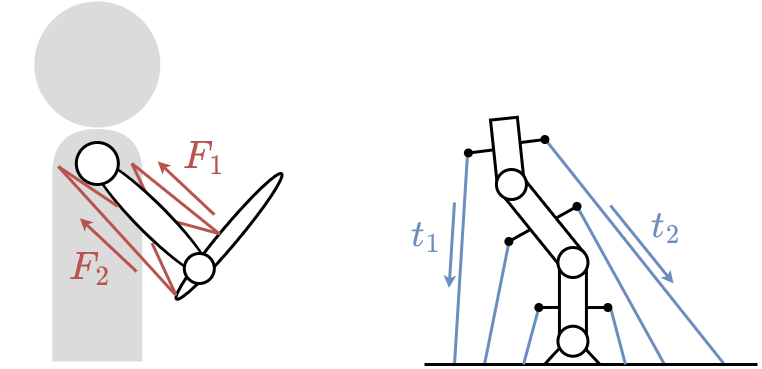
\includegraphics[width=\linewidth]{Chapters/imgs/muscle_mcdrs.png}
    \caption{An illustrative planar example of a human musculoskeletal model and a \gls{mcdr}. On the left human arm is modeled with two joints and six muscles, where each muscle can apply contraction forces $F_i$. On the right, a \gls{mcdr} robot is modeled with 3 joints and 6 cables, which can apply tension forces $t_i$.  }
    \label{fig:muscle_mcdrs}
\end{wrapfigure}




One of the main differences comes from the actuator point of view. When it comes to \glspl{mcdr}, the dynamics of the actuators is often neglected, considering them capable of instantaneously applying a range of $d$ tensile forces $\bm{t}\in\mathbb{R}^d$.
\begin{equation}
    \bm{t} \in [\bm{0},~\bm{t}_{max}]
\end{equation}
Additionally, this range is often considered constant and is not state dependent. For musculoskeleral models, on the other hand, the ranges of achievable muscle tension forces $\bm{F}$ are subject to many different biomechanical and biological factors, such as muscle length $\bm{l}$ and extension velocity $\dot{\bm{l}}$ as well the effects of fatigue and temperature.
Therefore the cables of the \glspl{mcdr} can be seen as idealised muscles which tensile force capacity stays constant. 

Consequently, the physical ability metrics defined for the musculoskeleral models have the same formulation as the ones used to asses the performance of \glspl{mcdr}.

\subsection{Wrench/Force polytope}
\label{ch:force_poly_human}
Task space force (or more generally wrench) capacity $\bm{f} \in \mathbb{R}^m$ is a well established metrics in biomechanics. It has been defined in two manners: a simplified formulation where the torques of $n$ human joints $\bm{\tau} \in \mathbb{R}^n$ are considered independent and limited (\ref{eq:human_torque_lim}) and in a more complete form where the human's joint torques $\bm{\tau}$ are generated by $d$ muscle tensile forces $\bm{F} \in \mathbb{R}^d$ which are limited in their respective ranges (\ref{eq:muslce_initial_range}).

Torque based polytopes \cite{rezzoug_application_2012,sasaki2011vertex} of achievable task space wrenches $\bm{f}$ have the same formulation as the force polytopes for robotic manipulators described in \Cref{ch:poly_force}. Therefore all the considerations for their evaluation are equivalent to those for robotic manipulators.  

However, real limits of human joint torques cannot be expressed as independent ranges (\ref{eq:human_torque_lim}) as they are generated by $d$ muscle tensile forces $\bm{F}$. The true limits of the joint torques $\bm{\tau}$ are polytope shaped as a consequence of the affine mapping of the muscle forces $\bm{F}$ to the \gls{js}, though the moment arm matrix $N(\bm{q})=-L(\bm{q})^T$.
\begin{equation}
\mathcal{P}_\tau(\bm{q}) = \{\bm{\tau} \in \mathbb{R}^n ~|~\bm{F}\in [\bm{F}_{min}, \bm{F}_{max}], ~\bm{\tau}=N(\bm{q})\bm{F}\}
\label{eq:poly_torque_human}
\end{equation}

The relationship of the achievable task space wrenches $\bm{f}$ and the joint torques $\bm{\tau}$ is described through the dynamics equation 
\begin{equation}
\underbrace{M(\bm{q})\ddot{\bm{q}} + C(\bm{q},\dot{\bm{q}})\dot{\bm{q}} + \bm{g}(\bm{q})}_{\bm{\tau}_b(\bm{q},\dot{\bm{q}},\ddot{\bm{q}})} + J^T(\bm{q})\bm{f} = \bm{\tau} 
\end{equation}
where $\bm{\tau}_b(\bm{q},\dot{\bm{q}},\ddot{\bm{q}})$ is a state dependant joint torque bias vector including the influence of the gravity $\bm{g}(\bm{q})$ and human state $\{\dot{\bm{q}},\ddot{\bm{q}}\}$ and the desired acceleration $\ddot{\bm{q}}$. 

Finally the achievable set of task space wrenches $\bm{f}\in\mathbb{R}^m$ can then be expressed as a set of all the achievable wrenches $\bm{f}$ given the polytope $\mathcal{P}_\tau$ shaped limits of joint torques $\bm{\tau}$
\begin{equation}
    \mathcal{P}_f(\bm{q},\dot{\bm{q}},\ddot{\bm{q}}) = \left\{ \bm{f} \in \mathbb{R}^m ~|~ \bm{\tau}\in \mathcal{P}_\tau(\bm{q}), ~~ J^T(\bm{q})\bm{f} = \bm{\tau} -\bm{\tau}_b(\bm{q},\dot{\bm{q}},\ddot{\bm{q}}) \right\}
    \label{eq:human_force_poly_ver_poly_lim}
\end{equation}
Or in its implicit formulation
\begin{equation}
    \mathcal{P}_f(\bm{q},\dot{\bm{q}},\ddot{\bm{q}}) = \left\{ \bm{f} \in \mathbb{R}^m ~|~ \bm{F}\in\left[\bm{F}_{min}, \bm{F}_{max} \right], ~~ \!J^T(\bm{q})\bm{f} =\! N(\bm{q})\bm{F} -\bm{\tau}_b(\bm{q},\dot{\bm{q}},\ddot{\bm{q}}) \right\}
    \label{eq:human_force_poly}
\end{equation}

The final polytope formulation $\mathcal{P}_f$ has an implicit form composed of two affine mappings. First the limits of the muscle tension forces $\bm{F}\in \mathbb{R}^d$ are projected into the limits of the joint torques $\bm{\tau}\in \mathbb{R}^n$, then the polytope of the joint torques $\mathcal{P}_\tau$ is transformed to the task space wrenches $\bm{f}\in \mathbb{R}^m$ using the Jacobian transpose matrix $J(\bm{q})^T$. As the musculoskeletal models often have large number of muscles $d$, the ending polytope $\mathcal{P}_f$ geometry is complex (having a large number of vertices and faces), both due to the number of muscles considered and the inherent complexity of the affine mapping. Therefore, this metric has been mostly used for static in-advance analysis of human postures \cite{hernandez_toward_2015}, due to its long execution times. 

However, \citet{carmichael_estimating_2013, carmichael2011Towards} have proposed a method capable of improving the time efficiency of the polytope resolution that has a potential to be used even in real-time applications. This method is based on \gls{rsm} that samples the polytope in a set of predefined direction in task space. By choosing the directions of interest in advance, the method is capable of approximating the polytope, however it does not give any guarantees on the approximation accuracy.

The achievable wrench polytope $\mathcal{P}_f$ formulation (\ref{eq:human_force_poly}) have been used for the analysis of the \glspl{mcdr} as well, for example in works by \citet{sheng2020operational} or \citet{Muralidharan2022}.

\subsection{Acceleration polytope}
\label{ch:human_aceleration_poly}

The task space acceleration polytope $\mathcal{P}_a$ describes the relationship between the limitation of the muscle tensile forces $\bm{F}\in \mathbb{R}^d$ and the set of achievable task space accelerations $\ddot{\bm{x}}\in\mathbb{R}^m$.

As in the case of the force polytope, the simplified approach to this metric is possible, where the human joint torque limits $\bm{\tau}\in\mathbb{R}^n$ are specified as independent ranges, resulting in the acceleration polytope formulation identical to the one for robotic manipulators, as introduced in \Cref{ch:accel_poly_robot}. 

However, human's joint torques $\bm{\tau}$ are not generated by a set of independent actuators, but with a set of $d$ contraction forces $\bm{F}$ produced by the muscle-tendon units $\bm{\tau}=N(\bm{q}) \bm{F}$. Therefore, real limits of achievable torques of human joints are polytope $\mathcal{P}_\tau$ shaped, as described by equation (\ref{eq:poly_torque_human}). 

The achievable acceleration polytope $\mathcal{P}_a$ formulation, respecting the muscle tension forces limits $\bm{F}$, can be derived from the human dynamics equation
\begin{equation}
M(\bm{q})\ddot{\bm{q}} + \underbrace{C(\bm{q},\dot{\bm{q}})\dot{\bm{q}} + \bm{g}(\bm{q}) + J^T(\bm{q})\bm{f}}_{\bm{\tau}_b(\bm{q},\dot{\bm{q}}, \bm{f})} = N(\bm{q}) \bm{F} 
\end{equation}
where $N(\bm{q})=-L(\bm{q})^T$ is the state dependant moment arm matrix. 
For any given human state $\{\bm{q},\dot{\bm{q}}, \bm{f}\}$, the effects of the human's motion, the gravity as well as the applied external wrenches, can be grouped in a constant torque vector $\bm{\tau}_b(\bm{q},\dot{\bm{q}},\bm{f})$. Then, the actuator acceleration $\ddot{\bm{q}}$ can be expressed was a function of the applied joint torque $\bm{\tau}$
\begin{equation}
    \ddot{\bm{q}} = M(\bm{q})^{-1}N(\bm{q})\bm{F} - M(\bm{q})^{-1}\bm{\tau}_b(\bm{q},\dot{\bm{q}}, \bm{f})
\end{equation}
Finally, the joint accelerations $\ddot{\bm{q}}$ can be transformed to the task space using the mapping (\ref{eq:js_to_cs_vaj_human:accel})
\begin{equation}
    \ddot{\bm{x}} = J(\bm{q})M(\bm{q})^{-1}N(\bm{q})\bm{F} - \underbrace{J(\bm{q})M(\bm{q})^{-1}\bm{\tau}_b(\bm{q},\dot{\bm{q}},\bm{f}) + \dot{J}(\bm{q}, \dot{\bm{q}})\dot{\bm{q}}}_{\bm{a}_b(\bm{q},\dot{\bm{q}},\bm{f})}
\end{equation}
where $\bm{a}_b(\bm{q},\dot{\bm{q}},\bm{f}) \in \mathbb{R}^m$ presents a constant bias vector for any human joint state $\{\bm{q},\dot{\bm{q}}\}$ and the generated external wrench $\bm{f}$. The polytope $\mathcal{P}_a$ of achievable task space accelerations $\ddot{\bm{x}}$ can then be expressed as
\begin{equation}
\begin{split}
    \mathcal{P}_a(\bm{q},\dot{\bm{q}},\bm{f}) = \{ \ddot{\bm{x}} \in \mathbb{R}^m ~|~ \bm{F}&\in\left[\bm{F}_{min}, \bm{F}_{max} \right],\\ \ddot{\bm{x}} &= J(\bm{q})M(\bm{q})^{-1}N(\bm{q})\bm{F} - \bm{a}_b(\bm{q},\dot{\bm{q}},\bm{f}) \}
\end{split}
\label{eq:poly_acceleration_hum}
\end{equation}
The polytope $\mathcal{P}_a$ is formulated as a linear and affine projection of the muscles tension force $\bm{F}$ limits using the state dependant projection matrix $J(\bm{q})M(\bm{q})^{-1}N(\bm{q})$.  This polytope is much simpler to resolve than the force polytope $\mathcal{P}_f$ as it represents a projection of the $d$ dimensional limits of muscle tension forces $\bm{F}$ to the lower $m$ dimensional space of achievable task space accelerations $\ddot{\bm{x}}$.

Polytope $\mathcal{P}_a$ metrics have been used for musculoskeletal model analysis of highly dynamical movements such as football throwing \cite{khatib2009robotics} and golf swinging \cite{demircan2012muscle}. Additionally this metric has been used for the design analysis of the \glspl{mcdr} as well \cite{sheng2020operational}.

\subsection{Velocity polytope}
\label{ch:human_vel_poly}
The simplest form of task space velocity capacity describes the relationship between the limited ranges (\ref{eq:human_js_vel_lim}) of human joint velocity $\dot{\bm{q}} \in \mathbb{R}^n$ and achievable task space velocities $\dot{\bm{x}} \in \mathbb{R}^m$, mapped through the Jacobian matrix $J(\bm{q}) \in \mathbb{R}^{m\times n}$.
\begin{equation}
    \mathcal{P}_v(\bm{q}) = \left\{ \dot{\bm{x}} \in \mathbb{R}^m ~|~ \dot{\bm{q}}\in\left[\dot{\bm{q}}_{min}, \dot{\bm{q}}_{max} \right], ~~ \dot{\bm{x}} = J(\bm{q})\dot{\bm{q}} \right\}
\end{equation}
This formulation is essentially the same as the one for robotic manipulators described in velocity \Cref{ch:vel_poly} and all the considerations discussed in that chapter are valid for this formulation as well.

However, taking in account only human's joint velocity $\dot{\bm{q}}$ limits in a form of independent ranges (\ref{eq:human_js_vel_lim}) does not take in consideration the limits of muscle extension velocity $\dot{\bm{l}}\in\mathbb{R}^d$. The true limits of human joint velocities are configuration dependent, as they are a consequence of the limits of muscle extension velocities $\dot{\bm{l}}$. The relationship between the joint and muscle extension velocities is given through the muscle Jacobian matrix $L(\bm{q}) \in \mathbb{R}^{d\times n}$, forming polytope shaped limits
\begin{equation}
    \mathcal{P}_{\dot{q}}(\bm{q}) = \left\{ \dot{\bm{q}} \in \mathbb{R}^n ~|~ \dot{\bm{l}}\in\big[\dot{\bm{l}}_{min}, \dot{\bm{l}}_{max} \big], ~~ L(\bm{q})\dot{\bm{q}} = \dot{\bm{l}} \right\}
    \label{eq:human_poly_joint_vel}
\end{equation}
These polytope shaped limits can then be used to define the achievable task space velocity $\dot{\bm{x}}\in \mathbb{R}^m$ polytope which respects the limits of the muscle extension velocity $\dot{\bm{l}}$.
\begin{equation}
    \mathcal{P}_v(\bm{q}) = \left\{ \dot{\bm{x}} \in \mathbb{R}^m ~|~ \dot{\bm{q}}\in  \mathcal{P}_{\dot{q}}(\bm{q}), ~~ J(\bm{q})\dot{\bm{q}} = \dot{\bm{x}} \right\}
    \label{eq:velocity_polytope_human_ver_poly_lim}
\end{equation}
Or in its implicit form
\begin{equation}
    \mathcal{P}_v(\bm{q}) = \left\{ \dot{\bm{x}} \in \mathbb{R}^m ~|~ \dot{\bm{l}}\in\big[\dot{\bm{l}}_{min}, \dot{\bm{l}}_{max} \big], ~~ J(\bm{q})\dot{\bm{q}} = \dot{\bm{x}}, ~~ L(\bm{q})\dot{\bm{q}} = \dot{\bm{l}} \right\}
    \label{eq:velocity_polytope_human}
\end{equation}

This metric has an implicit formulation making its resolution relatively complex, requiring using multiple standard methods for polytope evaluation. It first requires finding the limits of joint velocities $\dot{\bm{q}} \in \mathbb{R}^n$ based on the limits of the muscle extension velocities $\dot{\bm{l}} \in \mathbb{R}^d$ and then projecting them to the task space velocities $\dot{\bm{x}} \in \mathbb{R}^m$. 

To the best of our knowledge, polytope $\mathcal{P}_v$ in its full implicit form (\ref{eq:velocity_polytope_human}), has not yet been used with musculoskeletal models. However, this implicit formulation has been used for \glspl{mcdr} analysis \cite{Muralidharan2022}.

Simplified achievable velocity based physical ability metrics, such as manipulability ellipsoids, considering the joint velocity $\dot{\bm{q}}$ limits \cite{Chiu1988,petric2019assistive,Yang2017}, have been used in the human motion and ergonomics analysis. As these metrics neglect the muscle extension velocity $\dot{\bm{l}}$ limits, polytope $\mathcal{P}_v$ could be used as their more complete alternative. 

\subsection{Stiffness polytope}
\label{ch:human_stiffness_poly}
Stiffness metrics for human musculoskeletal models are used to evaluate the limitations of the endpoint displacement $\Delta x \in \mathbb{R}^m$ given the known muscle stiffness matrix $K_m \in \mathbb{R}^{d\times d}$ and a limited range of task space wrenches $\bm{f} \in \mathbb{R}^m$. 

\begin{equation}
    \bm{f}\in\left[\bm{f}_{min}, \bm{f}_{max} \right]
    \label{eq:force_stiff_range_human}
\end{equation}

With a known muscle stiffness matrix $K_m$, that can be determined using the Hill's muscle model \cite{LATASH1993653}, the joint stiffness matrix $K_j\in \mathbb{R}^{n\times n}$ can be found using the muscle Jacobian matrix $L(\bm{q}) \in \mathbb{R}^{d\times n}$
\begin{equation}
    K_j = L(\bm{q}) K_m L(\bm{q})^T 
\end{equation}
This \gls{js} stiffness matrix $K_j$ can be used to find the robot state dependent task space stiffness $K_c  \in \mathbb{R}^{m\times m}$, through the Jacobian matrix $J(\bm{q})\in\mathbb{R}^{m\times n}$  \cite{Salisbury1980,Ajoudani2018,Inouye2016}
\begin{equation}
     K_c(\bm{q})^{-1} = J(\bm{q}) K_j^{-1}J(\bm{q})^T
\end{equation}
Given the range of expected external wrenches (\ref{eq:force_stiff_range_human}), the polytope of maximal task space displacements $\Delta\bm{x}$ can then be expressed as
\begin{equation}
    \mathcal{P}_\Delta(\bm{q}) = \left\{ \Delta\bm{x} \in \mathbb{R}^m ~|~ \bm{f}\in\left[\bm{f}_{min}, \bm{f}_{max} \right], ~~ K_c(\bm{q})\Delta\bm{x} = \bm{f} \right\}
    \label{eq:stiffness_human_simple}
\end{equation}


However, this formulation considers that the external wrench $\bm{f}$ range (\ref{eq:force_stiff_range_human}) is inside the human wrench capacity. In order to make sure that the human's wrench capacity is not exceeded when calculating the maximal task space displacement polytope $\mathcal{P}_\Delta$ the external wrench range (\ref{eq:force_stiff_range_human}) needs to be intersected with the human's wrench polytope  $\mathcal{P}_f$ described in the \Cref{ch:force_poly_human}, the polytope $\mathcal{P}_\Delta$ of task space task space displacement $\Delta \bm{x}$ can then be expressed as
\begin{equation}
    \mathcal{P}_\Delta(\bm{q},\dot{\bm{q}},\ddot{\bm{q}}) = \left\{ \Delta\bm{x} \in \mathbb{R}^m ~|~ \bm{f}\in \left[\bm{f}_{min}, \bm{f}_{max} \right] \cap \mathcal{P}_f(\bm{q},\dot{\bm{q}},\ddot{\bm{q}}),  ~~ \! K_c(\bm{q})\Delta\bm{x}=\bm{f}\right\}
\end{equation}

If the maximal displacement polytope $\mathcal{P}_\Delta$ is calculated only in relationship to the human's wrench capacity $\mathcal{P}_f$, without specifying the expected range of external wrenches (\ref{eq:force_stiff_range_human}), this polytope can be expressed in an implicit form
\begin{equation}
\begin{split}
    \mathcal{P}_\Delta(\bm{q},\dot{\bm{q}},\ddot{\bm{q}}) =\! \{ \Delta\bm{x} \in \mathbb{R}^m ~|~\bm{F}\in\left[\bm{F}_{min}, \bm{F}_{max} \right]\!, \quad J^T(\bm{q})K_c(\bm{q})\Delta\bm{x}\!= N(\bm{q})\bm{F}\! -\! \bm{\tau}_b(\bm{q},\dot{\bm{q}},\ddot{\bm{q}}) \}\label{eq:stiffness_human_all}
\end{split}
\end{equation}
The stiffness polytope $\mathcal{P}_\Delta$ then represents the maximal task space displacement $\Delta \bm{x} \in \mathbb{R}^m$ that can be achieved given the human's muscle tensile forces $\bm{F} \in \mathbb{R}^d$ limits (\ref{eq:muslce_initial_range}), this polytope formulation is also called \textit{stiffness feasibility region} \cite{ajoudani2017choosing}.

The formulation of the polytope (\ref{eq:stiffness_human_simple}) has relatively low complexity, defined as a projection of the limits of the external task space wrenches $\bm{f} \in \mathbb{R}^m$ to the same dimensional task space displacements $\Delta \bm{x} \in \mathbb{R}^m$. However, the implicit polytope formulation (\ref{eq:stiffness_human_all}) is much more complex as the limits of muscle tension forces $\bm{F} \in \mathbb{R}^d$ first need to be projected to the limits of the joint torques $\bm{\tau} \in \mathbb{R}^n$ which in term determine the set of task space displacements $\Delta \bm{x} \in \mathbb{R}^m$. While the formulation  (\ref{eq:stiffness_human_simple}) can be resolved with standard polytope resolution algorithms, the formulation (\ref{eq:stiffness_human_all}) requires a combination of multiple methods, making it significantly more time consuming. 

These polytope based metrics however, to the best of our knowledge, have yet to be used with human musculoskeletal models and \glspl{mcdr}. However, their potential has already been shown for human posture analysis \cite{Inouye2016} and \gls{mcdr} design \cite{Ramadoss2021} applications, in their simplified ellipsoid forms.

\section{Polytope representation of collaboration abilities}
\label{ch:collab_metrics}

\begin{figure}[!h]
    \centering
    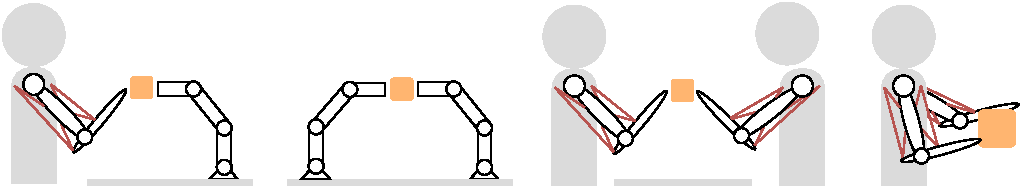
\includegraphics[width=\linewidth]{Chapters/imgs/collaboration.pdf}
    \caption{Illustrative examples of a common collaboration scenario composed of different actors (humans and robots), from left to right, human-robot, robot-robot, human-human and even two arms of a human subject can be seen as a collaboration of two musculoskeletal models.}
    \label{fig:collaboration_types}
\end{figure}

Physical ability metrics are an important tool for analysing how robots and humans comply with different requirements of tasks. In human-robot collaboration scenarios, these metrics can be used is to decide if the robot, or the human, is better suited to execute a certain task, by evaluating their different physical abilities (movement, forces, precision etc.) to the ones required by the task \cite{Edoardo2019Capability}. 

However, when it comes to the physical collaboration, where the task is executed jointly by the human and the robot physically interacting, expressing their common physical abilities is much more challenging. As their common physical ability is a combination of their individual abilities, to be able to calculate their common physical ability, they need to be expressed in a unified form.  

Many different physical abilities for humans and robots, can be represented in the polytope form, as described in \Cref{ch:robot_metrics} and \Cref{ch:human_metrics}. Expressing their physical abilities in this unifying form enables using different efficient tools from the polytope algebra to combine their individual polytopes, such as Minkowski sums, intersections and convex-hulls.
Therefore, given their individual polytopes of different physical abilities and the physics of their physical interaction scenario, different polytope algebra operations can be leveraged to express their common physical ability in the polytope form as well.

One example of such characterisation has been developed by \citet{lee2001velocity}, showing how polytopes can be used to describe the common velocity capacity of multi-arm collaborative robotic system, by intersecting their individual polytopes. However, this approach is yet to be used for characterising the common capacity of the human-robot interaction, as well as to be extended to other physical abilities and other collaboration scenarios. 


Therefore, following sections describe the characterisation of different common physical abilities of the human-robot interaction, based on one classical example of human-robot collaboration scenario, where the two actors interact physically to manipulate an object that is rigidly fixed in the end-effector of the robot and in the hand of the human. First, \Cref{ch:which_metric_which} introduces the physical relationships describing this collaboration scenario, followed by \Cref{ch:force_collab} and \Cref{ch:velocity_collab}, giving more specific examples of how these relationships are exploited to calculate the common force and velocity capacity of a physical human-robot collaboration leveraging the polytope algebra. 
Different versions of this scenario are shown on \Cref{fig:collaboration_types}, ranging from human-robot interaction to the interaction of the two arms of a human subject, that can be seen as two separate musculoskeletal models collaborating.

% \todos{Even though the following sections are focusing on one collaboration scenario, similar approach can be used to characterising any other collaboration scenario as well.}

\subsection{Human-robot collaboration scenario}
\label{ch:which_metric_which}

A classical human-robot physical interaction scenario is considered, where the human operator and the robot are physically interacting in order to manipulate an object which is rigidly fixed both in the robot's end-effector and the human's hand. A simplified view of this collaboration scenario is shown on \Cref{fig:table_inter}, while a more general view of this scenario, with different actors (humans and robots), is shown on \Cref{fig:collaboration_types}.

\begin{wrapfigure}{r}{0.5\textwidth}
    \centering
    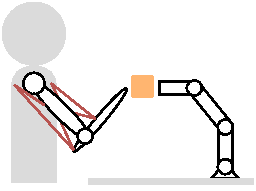
\includegraphics{Chapters/imgs/example_inter.pdf}
    \caption{A collaborative example scenario where a human and a robot interact over an object fixed rigidly in the end-effector of the robot and in the hand of the human.}
    \label{fig:table_inter}
\end{wrapfigure}
When it comes to commonly manipulating an object held by both human and the robot, the supposition of rigid contact with the object can be used to formulate the force equilibrium equation and the relative motion constraints \cite{Prattichizzo2016}. 

As they both apply forces on the object, the resulting force $\bm{f}$ the object will exert on the environment (if in contact with it) or transform into motion follows from the force equilibrium ( sum of all forces $\bm{f}_i$ is equal to zero ), and is equal to the sum of the applied forces by the robot $\bm{f}_r$ and the human $\bm{f}_h$. 
\begin{equation}
    \bm{f} = \bm{f}_r + \bm{f}_h, \qquad  m_o\ddot{\bm{x}} = \bm{f} 
\end{equation}
If the object is not in contact with the environment, the force $\bm{f}$ will generate object's acceleration $\ddot{\bm{x}}$  in space proportional to its mass $m_o$.

Furthermore, as the object is rigidly attached to both robot and the human, there is no relative movement possible between the object, human's hand and robot's end-effector. According to this condition, the movement of the object (position $\bm{x}$, velocity $\dot{\bm{x}}$, acceleration $\ddot{\bm{x}}$, jerk $\dddot{\bm{x}}$, etc.) is equivalent to the movement of both the human's hand $\{\bm{x}_h,\dot{\bm{x}}_h,\ddot{\bm{x}}_h,\dddot{\bm{x}}_h\}$ and the robot's end-effector $\{\bm{x}_r,\dot{\bm{x}}_r,\ddot{\bm{x}}_r,\dddot{\bm{x}}_r\}$.
\begin{equation}
    {\bm{x}}_h={\bm{x}}_r={\bm{x}}, \qquad
    \dot{\bm{x}}_h=\dot{\bm{x}}_r=\dot{\bm{x}}, \qquad
    \ddot{\bm{x}}_h=\ddot{\bm{x}}_r=\ddot{\bm{x}}, \qquad
    \dddot{\bm{x}}_h=\dddot{\bm{x}}_r=\dddot{\bm{x}}
    \label{eq:kinematic_condition_contact}
\end{equation}

These two relationships, considering the rigid contact between the robot, human and the object, can be used to describe different physical abilities of the human-robot collaboration in the described scenario. \Cref{ch:force_collab} describes exploiting this relationship to calculate the common force capacity while \Cref{ch:velocity_collab} described the calculation of their common velocity capacity.


% where each one of the forces is bounded in withing the polytope $\bm{f}_i \in \mathcal{P}_{fi}$. 
% \begin{equation}
%     \mathcal{P}_f = \{\bm{f}\in \mathbb{R}^m ~|~\bm{f} = \bm{f}_r + \bm{f}_h , \quad\bm{f}_r \in \mathcal{P}_{fr},~\bm{f}_h \in \mathcal{P}_{fh}\}
% \end{equation}
% Therefore their common wrench capacity can be expressed as a sum of their individual wrench capacities, corresponding to the Minkowski sum $\oplus$ in polytope algebra 
% \begin{equation}
%     \mathcal{P}_f = \mathcal{P}_{fr}\oplus \mathcal{P}_{fh}
% \end{equation}


% %the maximal velocity capacity of the object will be limited by the actor (human or robot) with the least velocity capacity. 

% On the other hand, in the proposed collaboration scenario, as both robot and the human are rigidly attached to the object, the velocity of the object $\dot{\bm{x}}$ is equal to the velocity of the human's hand $\dot{\bm{x}}_h$ and the robot's end-effector $\dot{\bm{x}}_r$ \cite{Prattichizzo2016}
% \begin{equation}
%     \dot{\bm{x}}_h=\dot{\bm{x}}_r=\dot{\bm{x}}
%     \label{eq:kinematic_condition_contact}
% \end{equation}
% as both of them have their own limited velocity capacity $\dot{\bm{x}}_h \in \mathcal{P}_{vh},\dot{\bm{x}}_r \in \mathcal{P}_{vr}$ the object velocity has to respect all of them
% \begin{equation}
%     \mathcal{P}_v = \{\dot{\bm{x}}\in \mathbb{R}^m ~|~ \dot{\bm{x}} \in \mathcal{P}_{vr},~\dot{\bm{x}} \in \mathcal{P}_{vh}\}
% \end{equation}
% Geometrically, this operation can be represented as an intersection of their velocity capacities, and the intersection $\cap$ operation can be calculated efficiently using polytope algebra. 
% \begin{equation}
%     \mathcal{P}_v =  \mathcal{P}_{vh} \cap \mathcal{P}_{vr}
% \end{equation}



% More generally, all the polytope formulations that require calculating the wrench/force capacity, for both robot's and human's, will be combined using Minkowski sum $\oplus$. Such metrics are human's and robot's wrench/force polytope and stiffness region polytope.

% More generally, all polytope metrics characterising robot's or human's movement capacity (velocity $\dot{\bm{x}}$, acceleration $\ddot{\bm{x}}$, etc.) will be subject to the same condition (\ref{eq:kinematic_condition_contact}) and will be combined using the intersection $\cap$ operation.




% The further discussed procedures for calculating joint physical ability polytopes are valid for the considered collaboration scenario (showed on \Cref{fig:table_inter} or more generally on \Cref{fig:collaboration_types}), however the same methodology can be used to any other collaboration scenario as well.

% \begin{table}
% \centering
% \begin{tabular}{|l|c | c| c| c|}
% \hline
% Polytope Metric & Equation & Dynamics & Collaboration operator \\
% \hline
%  \multicolumn{5}{c}{Robotic manipulators }  \\
% \hline
% Velocity  &  \ref{eq:poly_vel_rob}& No & $\cap$ \\
% Kinematic Acceleration  & \ref{eq:poly_accel_kin} & No & $\cap$ \\
% Kinematic Jerk  &  \ref{eq:poly_jerk_kin}& No &  $\cap$ \\
% Precision  & \ref{eq:poly_precision_rob} & No&  $\cap$ \\
% Force/Wrench  & \ref{eq:poly_force_rob} & Yes &$\oplus$ \\
% Acceleration  & \ref{eq:pol_accleration_rob} & Yes &   $\cap$ \\
% Stiffness feasibility  &  \ref{eq:pol_sfr_rob} & Yes& $\oplus$ \\
% \hline
%  \multicolumn{5}{c}{Human musculoskeletal models}  \\
% \hline
% Velocity  & \ref{eq:velocity_polytope_human} & No &  $\cap$ \\
% Force/Wrench & \ref{eq:human_force_poly} & Yes & $\oplus$ \\
% Acceleration  & \ref{eq:poly_acceleration_hum} & Yes &  $\cap$ \\
% Stiffness feasibility  & \ref{eq:stiffness_human_all}  & Yes&  $\oplus$ \\
% \hline
% \end{tabular}
% \caption{The list of common polytope based physical ability metrics alongside their polytope algebra operator for the example collaborative scenario (\Cref{fig:table_inter}), as well as the indication of their capacity to account for the dynamics effects.}
% \label{tab:table_comparisson_colloboration}
% \end{table}


\subsection{Force polytope}
\label{ch:force_collab}
\begin{figure}[!h]
    \centering
    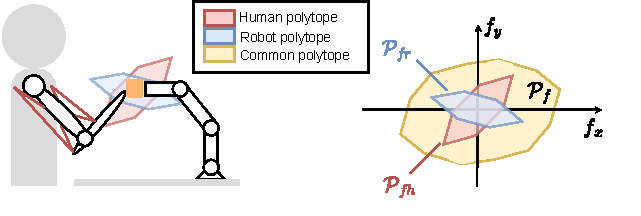
\includegraphics[width=0.7\linewidth]{Chapters/imgs/force_collab.pdf}
    \caption{A collaborative example scenario where a human and a robot interact over an object fixed rigidly in the end-effector of the robot and in the hand of the human. The force polytope of the human (red) and the robot (blue) as well as their collaborative polytope (orange) calculated as a Minkowski sum of their individual polytopes are shown on the right.}
    \label{fig:collaboration_force}
\end{figure}

When a human operator and a robot are physically interacting in order to manipulate an object, which is rigidly fixed both in the robot's end-effector and the human hand, the final force exerted on the object will be the sum of the forces of the human $\bm{f}_h$ and the force of the robot $\bm{f}_r$.
\begin{equation}
    \bm{f} = \bm{f}_h + \bm{f}_r
\end{equation}

Their individual force capacity can be expressed in a polytope form, for the human  $\mathcal{P}_{fh}$ and the robot  $\mathcal{P}_{fr}$ respectively. Finally, as their forces acting on the object are summed, their common force capacity on the object can be expressed as
\begin{equation}
    \mathcal{P}_f = \{\bm{f}\in \mathbb{R}^m ~|~\bm{f} = \bm{f}_r + \bm{f}_h , \quad\bm{f}_r \in \mathcal{P}_{fr},~\bm{f}_h \in \mathcal{P}_{fh}\}
\end{equation}
Therefore their common wrench capacity can be expressed as a sum of their individual wrench capacities, corresponding to the Minkowski sum $\oplus$ in polytope algebra 
\begin{equation}
    \mathcal{P}_f = \mathcal{P}_{fr}\oplus \mathcal{P}_{fh}
\end{equation}

A planar example of this collaboration scenario and the polytopes obtained is in shown on \Cref{fig:collaboration_force}. 

In more general case, if a collaboration is composed of $N$ actors rigidly holding an object, where their force capacity is expressed in a polytope form $\mathcal{P}_{fi}$, then their common force capacity can be calculated as the Minkowski sum of the $N$ polytopes.

\begin{equation}
    \mathcal{P}_f =  \mathcal{P}_{f1} \oplus \mathcal{P}_{f2} \oplus ~\ldots ~\oplus  \mathcal{P}_{fN}
\end{equation}

Furthermore, the polytope formulations that require calculating the wrench/force capacity, for both robot's and human's, will be combined using Minkowski sum $\oplus$. Such metrics are human's and robot's wrench/force polytope and stiffness region polytope, as shown in \Cref{tab:merged_table}.

\subsection{Velocity polytope}
\label{ch:velocity_collab}

\begin{figure}[!h]
    \centering
    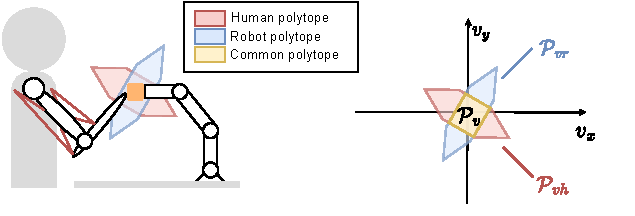
\includegraphics[width=0.7\linewidth]{Chapters/imgs/velocity_collab.pdf}
    \caption{A collaborative example scenario where a human and a robot interact over an object fixed rigidly in the end-effector of the robot and in the hand of the human. The velocity polytope of the human (red) and the robot (blue) as well as their collaborative polytope (orange) calculated as an intersection of their individual polytopes are shown on the right.}
    \label{fig:collaboration_vel}
\end{figure}

When a human operator and a robot are physically interacting in order to manipulate an object which is rigidly fixed both in the robot's end effector and the human hand, there is no relative movement of the object with respect to the human's hand and the robot's end effector
\begin{equation}
    \dot{\bm{x}}_h=\dot{\bm{x}}_r=\dot{\bm{x}},
\end{equation}

Once their individual velocity capacity is expressed in polytope form $\mathcal{P}_{vh}$ and $\mathcal{P}_{vr}$, their common velocity capacity $\mathcal{P}_v$ (the achievable velocities of the object) can then be calculated as 
\begin{equation}
    \mathcal{P}_v = \{\dot{\bm{x}}\in \mathbb{R}^m ~|~ \dot{\bm{x}} \in \mathcal{P}_{vr},~\dot{\bm{x}} \in \mathcal{P}_{vh}\}
\end{equation}
Geometrically, this operation can be represented as an intersection of their velocity capacities, and the intersection $\cap$ operation can be calculated efficiently using polytope algebra. 
\begin{equation}
    \mathcal{P}_v =  \mathcal{P}_{vh} \cap \mathcal{P}_{vr}
\end{equation}

A planar example of this collaboration scenario and the polytopes obtained is in shown on \Cref{fig:collaboration_vel}. 


% The maximal velocity the object can achieve in a certain direction $\bm{v}_{max}$ will be limited by the actor who has the lower maximal velocity in that direction. It can be found as the minimum value of the maximal velocity the human arm can achieve $\bm{v}_{h,max}$ and the robot's end-effector can achieve $\bm{v}_{r,max}$
% \begin{equation}
%     \bm{v}_{max}= \min \{\bm{v}_{h,max}, \bm{v}_{r,max}\}
% \end{equation}

In a more general case where there are $N$ actors (robots and humans) collaborating by rigidly holding the object, and where their velocity capacity is expressed in a polytope form $\mathcal{P}_{vi}$, the common velocity capacity can be calculated as their intersection
\begin{equation}
    \mathcal{P}_v =  \mathcal{P}_{v1} \cap \mathcal{P}_{v2} \cap ~~ \ldots ~~\cap \mathcal{P}_{vN}
\end{equation}

Furthermore, the polytope formulations characterising robot's or human's movement capacity (velocity $\dot{\bm{x}}$, acceleration $\ddot{\bm{x}}$, etc.) will be subject to the same condition (\ref{eq:kinematic_condition_contact}) and will be combined using the intersection $\cap$ operation, as shown in \Cref{tab:merged_table}.

\section{Conclusion and synthesis}
\label{ch:collab_metrics_overview}

This chapter brings an overview of the polytope based physical ability characterisations for humans and robots, with the aim to develop a unified view of their abilities and provide a base for characterising their common physical abilities. As described in \Cref{ch:inro_overview}, the literature proposes many different metrics for quantifying human and robot physical abilities. However, they are often very different in scope, accuracy, physical interpretation and in many cases specific to only robots or only humans. The focus of this chapter, as well as this thesis, is therefore placed on polytope based representations of physical abilities as they are arguably the most complete and the most accurate characterisations for both robots and humans, based on their musculoskeletal models.

This chapter brings an overview of the common polytope based representations of humans' and robots' physical abilities in \Cref{ch:robot_metrics} and \Cref{ch:human_metrics}, in the attempt to present a systematic view on their formulations. In this overview, different physical abilities of humans (based on musculoskeletal models) and robots are characterised by finding the relationships between their actuation limits and the achievable sets of different task-related variables. As these relationships are usually described through their highly nonlinear dynamics and kinematics relationships, in order to obtain the polytope-shaped representations, the dynamics and kinematics equations are linearised around a specific state. This approach yields linear and affine transformations of the actuator limits to the achievable sets of desired task space variables.

Common polytope formulations, described in \Cref{ch:robot_metrics} for robots and in \Cref{ch:human_metrics} for humans, involve different linearised dynamics and kinematics equations, as well as different actuation limits. However, they can be represented using a generic formulation
\begin{equation}
    \mathcal{P}_x = \{\bm{x}\in\mathbb{R}^m ~|~ A\bm{x}=B\bm{y} + \bm{b}, ~ \bm{y}\in\mathcal{P}_y\}
    \label{eq:generic_polyt_view}
\end{equation}
where the polytope $\mathcal{P}_x$ represents the achievable set of the task space variable $\bm{x}\in\mathbb{R}^m$, $\bm{y}\in\mathbb{R}^k$ is the input (actuator) variable limited within input set (actuator limits) $\mathcal{P}_y$. The input set $\mathcal{P}_y$ is often defined in the form of intervals of different input (actuator) variables, however in general case it can have a polytope shape as well. The linearised dynamics and kinematics equations can be represented, in a generic case, using the equation $A\bm{x}\!=\!B\bm{y}\!+\!\bm{b}$, where the matrix $A\in\mathbb{R}^{k\times m}$ is a linear transformation matrix from the $m$ dimensional output (task) space to the $k$ dimensional intermediate space, the matrix $B\in\mathbb{R}^{k\times d}$ is a transformation matrix from the $n$ dimensional input space to the intermediate space and $\bm{b}\in\mathbb{R}^k$ is a bias vector expressed in the intermediate space. Furthermore, the dimension of output (task) space $m$ is lower than the intermediate space dimension $k\!\geq\! m$ , which is in term lower than the input (actuator) space dimension $n\!\geq\! k\!\geq\! m$. This condition comes from the fact that when characterising the physical abilities, the polytopes map higher dimensional input space (ex. \gls{js} or muscle force space) to the lower dimensional output space (ex. \gls{cs}).

\begin{table}[!b]
% \hspace{-1cm}
\scalefont{0.9}
\centering
\begin{tabular}{|l|c|c|c|c|c|c|c|c|c|}
\hline
Polytope capacity & Eqn. & $\bm{x}$ & $A$ & $B$ & $\bm{y}$ & Input set $\mathcal{P}_y$ & $\bm{b}$ & Cond. & Collab. \\
\hline
\multicolumn{10}{c}{Robotic manipulators} \\
\hline
Velocity & \ref{eq:poly_vel_rob}& $\dot{\bm{x}}$ & $I_{m\times m}$ & $J$ & $\dot{\bm{q}}$& $[\dot{\bm{q}}_{min},\dot{\bm{q}}_{max}]$ & - & Kin & $\cap$ \\
Kin. Acceleration & \ref{eq:poly_accel_kin} & $\ddot{\bm{x}}$ & $I_{m\times m}$ & $J$ & $\ddot{\bm{q}}$ & $[\ddot{\bm{q}}_{min},\ddot{\bm{q}}_{max}]$ & $\bm{a}_b$ & Kin & $\cap$ \\
Kin. Jerk &\ref{eq:poly_jerk_kin} & $\dddot{\bm{x}}$ & $I_{m\times m}$ & $J$ & $\dddot{\bm{q}}$& $[\dddot{\bm{q}}_{min},\dddot{\bm{q}}_{max}]$ & $\bm{j}_b$ & Kin & $\cap$ \\
Precision & \ref{eq:poly_precision_rob} & $\delta\dot{\bm{x}}$ & $I_{m\times m}$ & $J$ & $\delta\bm{q}$ &$[\delta{\bm{q}}_{min},\delta{\bm{q}}_{max}]$ & - & Kin & $\cap$ \\
Force/Wrench & \ref{eq:poly_force_rob} & $\bm{f}$ & $J^T$ & $I_{n\times n}$ & $\bm{\tau}$ &$[\bm{\tau}_{min},\bm{\tau}_{max}]$ & -$\bm{\tau}_b$ & Dyn & $\oplus$ \\
Acceleration & \ref{eq:pol_accleration_rob} & $\ddot{\bm{x}}$ & $I_{m\times m}$ & $JM^{-1}$ & $\bm{\tau}$ &$[\bm{\tau}_{min},\bm{\tau}_{max}]$ & -$\bm{a}_b$ & Dyn & $\cap$ \\
Stiffness & \ref{eq:pol_sfr_rob}& $\Delta\bm{x}$ & $J^TK_c$ & $I_{n\times n}$ & $\bm{\tau}$ &$[\bm{\tau}_{min},\bm{\tau}_{max}]$ & -$\bm{\tau}_b$ & Dyn & $\oplus$ \\
\hline
\multicolumn{10}{c}{Human musculoskeletal models} \\
\hline
Velocity &\ref{eq:velocity_polytope_human} & $\dot{\bm{x}}$ & $I_{m\times m}$ & $J$ & $\dot{\bm{q}}$ & $\mathcal{P}{\dot{\bm{q}}}$ & - & Kin & $\cap$ \\
Force/Wrench & \ref{eq:human_force_poly} & $\bm{f}$ & $J^T$ & $N$ & $\bm{F}$ & $[\bm{F}_{min},\bm{F}_{max}]$ & -$\bm{\tau}_b$ & Dyn & $\oplus$ \\
Acceleration & \ref{eq:poly_acceleration_hum} & $\ddot{\bm{x}}$ & $I_{m\times m}$ & $JM^{-1}N$ & $\bm{F}$ & $[\bm{F}_{min},\bm{F}_{max}]$ & -$\bm{a}_b$ & Dyn & $\cap$ \\
Stiffness & \ref{eq:stiffness_human_all} &$\Delta\bm{x}$ & $J^TK_c$ & $N$ & $\bm{F}$ & $[\bm{F}_{min},\bm{F}_{max}]$ & -$\bm{\tau}_b$ & Dyn & $\oplus$ \\
\hline
\end{tabular}
\caption{The list of common polytope formulations for characterising physical abilities of robots and humans introduced in \Cref{ch:robot_metrics} and \Cref{ch:human_metrics} respectively. The table shows the correspondence of the common formulations to the generic formulation described by the equation (\ref{eq:generic_polyt_view}). The table further specifies if the polytope formulations is specified in kinematic or dynamic conditions. Finally, the table shows the necessary polytope algebra operator in order to characterise the common abilities in the collaboration scenario described in \Cref{ch:which_metric_which}.}
\label{tab:merged_table}
\end{table}

\Cref{tab:merged_table} brings a list of the polytope formulations for robots and humans, introduced in \Cref{ch:robot_metrics} and \Cref{ch:human_metrics} respectively, in a condensed view. The table shows how different polytope formulations correspond with the generic polytope formulation (\ref{eq:generic_polyt_view}), in terms of system matrices $A,B$, input, output and bias vectors $\bm{x},\bm{y},\bm{b}$ and the input limits $\mathcal{P}_y$.

Polytopes, apart from being able to accurately represent both human's and robot's physical abilities, enable combining their individual polytopes for characterising the common physical abilities when interacting physically to execute different task. Given the physical ability of interest and the physics of the human-robot physical interaction scenario, different polytope algebra tools, such as Minkowski sum or intersection, can be used to express the common physical ability of their interaction in the polytope form as well.


\Cref{ch:collab_metrics}, demonstrates the use of different polytope algebra operations to characterise force and movement capacity of the human-robot collaboration in one classical collaboration scenario, where the human and the robot jointly manipulate an object. In the context of the same scenario, \Cref{tab:merged_table} shows the polytope algebra operators (Minkowski sum $\oplus$ and intersection $\cap$) used to combine their individual polytopes to characterise their different physical abilities as one system.


In summary, polytopes enable accurate representation of human's and robot's physical abilities, as well as characterising their common physical abilities when collaborating physically to execute a task. In that way, this representation provides tools to create more advanced collaboration scenarios. 
Accurate representation of robot's physical abilities enables exploiting its abilities fully when designing its tasks, creating the adapted robot control strategies or planning for its trajectories. On the other hand, accurate representation of human's abilities enables assessing the task ergonomics and making sure that human's capacity is never surpassed. Additionally, it enables creating more human-centered robot behaviours, where the robot adapts its assistance level to the lacking physical abilities of the human operator. 
Finally, a unified representation of their individual and common physical abilities might enable new task scheduling techniques capable of assessing if different tasks are more suitable for robots, human operators or are they more suitable for their collaboration. 

However, polytope formulations, as introduced in \Cref{ch:robot_metrics} and \Cref{ch:human_metrics}, need to be transformed to more standard representations in order to  be used in practical implementations. The two most common ways to represent a polytope are as a set of vertices, or as a set of inequality constraints corresponding to its faces. Depending on the polytope formulation structure different transformation strategies, to the one of these forms, need to be employed, where the computational efficiency of the transformation operation can vary significantly with respect to the formulation complexity. Therefore, the following chapter (\Cref{ch:transformin_polytopes}) focuses on providing a generic view on different formulation families present when characterising physical abilities of humans and robots, with the aim to specify different polytope transformation strategies applicable to each of the families as well as to discuss their computational complexity.
